\documentclass[9pt]{beamer}

\usepackage[utf8]{inputenc}
\usepackage[T1]{fontenc}
\usepackage[french]{babel}
\usepackage[ddmmyyyy]{datetime}
\usepackage{listings,lstautogobble,graphicx}

\renewcommand{\rmdefault}{\sfdefault} %Utilisation de la police sans-serif ("Computer Modern Sans") pour la police roman
\renewcommand{\ttdefault}{pcr} 	%Utilisation d'une police "CourrierNew" pour la police monospaced (pour faire un listing manuel)

\usetheme{Warsaw}
\useinnertheme{rectangles}
\setbeamerfont{headline}{size=\large}
\setbeamerfont{frametitle}{size=\normalsize}


%Plan/Sommaire automatique avant chaque section
\AtBeginSection[]{
  \begin{frame}
  \frametitle{Plan}
  \tableofcontents[currentsection]
  \end{frame}
}

\definecolor{darkgreen}{rgb}{0.1,0.5,0.1}
\definecolor{mygray}{rgb}{0.93,0.93,0.93}
\definecolor{mymauve}{rgb}{0.58,0,0.82}
\lstset{	
	language=C,
	basicstyle=\small\ttfamily,
	backgroundcolor=\color{mygray},
	breaklines=true,
	breakatwhitespace=true,
	tabsize=3,
	captionpos=b,
	frame=none,
	rulecolor=\color{black},
	keywordstyle=\color{blue}\bfseries,
	stringstyle=\color{orange},
	showstringspaces=false,
	commentstyle=\footnotesize\color{darkgreen},
	keepspaces=true,
	extendedchars=true,
	numbers=left,
	numberstyle=\tiny\color{lightgray},
	stepnumber=1,
	escapeinside={(@}{@)},
	autogobble=true,
	literate=
		{á}{{\'a}}1 {é}{{\'e}}1 {í}{{}}1 {ó}{{\'o}}1 {ú}{{\'u}}1
		{Á}{{\'A}}1 {É}{{\'E}}1 {Í}{{\'I}}1 {Ó}{{\'O}}1 {Ú}{{\'U}}1
		{à}{{\`a}}1 {è}{{\`e}}1 {ì}{{\`i}}1 {ò}{{\`o}}1 {ù}{{\`u}}1
		{À}{{\`A}}1 {È}{{\'E}}1 {Ì}{{\`I}}1 {Ò}{{\`O}}1 {Ù}{{\`U}}1
		{ä}{{\"a}}1 {ë}{{\"e}}1 {ï}{{\"i}}1 {ö}{{\"o}}1 {ü}{{\"u}}1
		{Ä}{{\"A}}1 {Ë}{{\"E}}1 {Ï}{{\"I}}1 {Ö}{{\"O}}1 {Ü}{{\"U}}1
		{â}{{\^a}}1 {ê}{{\^e}}1 {î}{{\^i}}1 {ô}{{\^o}}1 {û}{{\^u}}1
		{Â}{{\^A}}1 {Ê}{{\^E}}1 {Î}{{\^I}}1 {Ô}{{\^O}}1 {Û}{{\^U}}1
		{œ}{{\oe}}1 {Œ}{{\OE}}1 {æ}{{\ae}}1 {Æ}{{\AE}}1 {ß}{{\ss}}1
		{ç}{{\c c}}1 {Ç}{{\c C}}1 {ø}{{\o}}1 {å}{{\r a}}1 {Å}{{\r A}}1
		{€}{{e}}1 {£}{{\pounds}}1 {«}{{\guillemotleft}}1
		{»}{{\guillemotright}}1 {ñ}{{\~n}}1 {Ñ}{{\~N}}1 {¿}{{?`}}1
}

\author{Steve Alabi - Taha Bendjeddou - Younes Benyamna - Malek Zemni}
\institute{M2 SeCReTS - UVSQ}
\date{\today}
\usepackage{myInfolines}
\usepackage{longtable,array}
\title{Programmation système}


\begin{document}

	\begin{frame}
		\titlepage
	\end{frame}
	
	\begin{frame}
		\tableofcontents
	\end{frame}
	
	\section{Introduction}
	\subsection{Systèmes d'exploitation}
		\begin{frame}
			\begin{block}{Système d'exploitation}
			Ensemble de programmes qui dirigent l'utilisation des capacités d’un ordinateur par des logiciels applicatifs.\\
			Il reçoit des demandes d'utilisation des capacités de l'ordinateur (stockage des mémoires et des disques durs, calcul du processeur, communication vers des périphériques ou via le réseau) de la part des logiciels applicatifs.\\
			Le système d'exploitation accepte ou refuse ces demandes, puis réserve les ressources en question pour éviter que leur utilisation n'interfère avec d'autres demandes provenant d'autres logiciels.
			\end{block}
			
			\begin{center}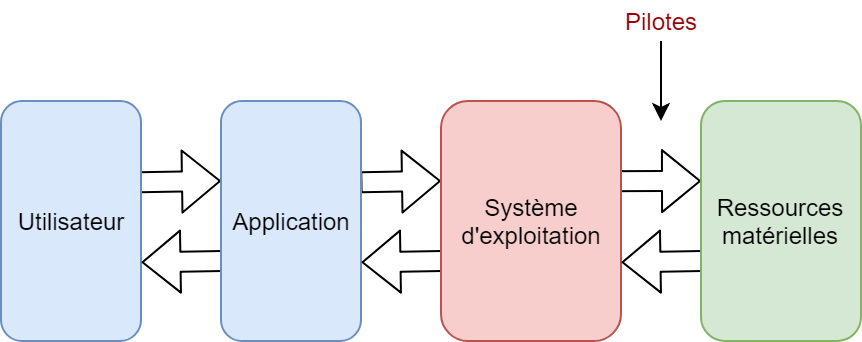
\includegraphics[scale=0.3]{img/SE.png}\end{center}
		\end{frame}
		
		\begin{frame}
			-> dissocier les programmes et le matériel, afin notamment d'assurer la \textbf{gestion des ressources} et offrir à l'utilisateur une interface homme-machine simplifiée lui permettant de s'affranchir de la complexité de la machine physique.
			\\~\\
			\textbf{Composantes d'un système d'exploitation :}~\\
				\begin {itemize}
					\item \textbf{Noyau (kernel) :} représente les fonctions fondamentales du système, gère les ressources de l’ordinateur et permet aux différents composants — matériels et logiciels — de communiquer entre eux.
					\item \textbf{L'interpréteur de commande (shell) :} permet la communication avec le système d'exploitation par l'intermédiaire d'un langage de commandes.
					\item \textbf{Le système de fichiers :} permet d'enregistrer les fichiers dans une arborescence.
				\end{itemize}
		\end{frame}
	
	\subsection{Programmation système}
		\begin{frame}
			\textbf{Programmation système :}
			\\~\\
			Type de programmation qui vise au développement de programmes qui font partie du système d’exploitation d’un ordinateur ou qui en réalisent les fonctions.\\~\\
			
			Elle se distingue de la \textit{\textbf{programmation des applications}} en ce qu’elle s’intéresse non pas au traitement des données, mais à la résolution des problèmes pour les humains, aux interfaces (API), aux protocoles (communication) et à la gestion des ressources.\\~\\
			
			En réalité, seuls les \textit{\textbf{programmes d'application}} sont utilisés pas les utilisateurs. Les \textit{\textbf{programmes système}} le sont implicitement.\\~\\
			
			La programmation système inclut, en outre, l’accès aux fichiers, la gestion de la mémoire vive et des processeurs et la programmation de tous les périphériques qui font entrer ou sortir de l’information d’un ordinateur (clavier, écran, modems...). Elle permet donc de communiquer avec ces périphériques, créer des pilotes, voire même créer un système d'exploitation.
			
		\end{frame}
		
		\begin{frame}
			\textbf{Sous UNIX :}
			\\~\\
			90\% du code est écrit en \textit{\textbf{langage C}} (qui a été spécialement créé pour le développement du système UNIX), le reste est écrit en assembleur.
			\\~\\
			- \textit{\textbf{couche logicielle} : } regroupe tous les programmes qui fournissent des services similaires.\\ 
			- \textit{\textbf{couche d'abstraction matérielle} : } une couche logicielle qui a accès au matériel informatique.
			\\~\\
			-> Le \textit{\textbf{noyau}} est une sorte de logiciel d'arrière-plan qui assure les communications entre ces programmes. C'est donc par lui qu'il va falloir passer pour avoir accès aux informations du système.
			\\~\\
			\textbf{Appels-systèmes :} fonctions qui permettent de communiquer avec le noyau depuis l’espace utilisateur, en demandant des services ou des ressources au système.
		\end{frame}		
		
	\section{Gestion d'erreurs}
	\subsection{Les flux}
		\begin{frame}
			\textbf{Les flux :}
			\\~\\
			Les flux peuvent être représentés comme des canaux dans lesquels circulent des informations. Ces flux sont représentés par l'abstraction de base du disque dur : le fichier. Ainsi, tout ce qui sera écrit dans un des flux sera écrit dans le fichier associé.
			\\~\\
			\begin{itemize}
				\item le flux d'entrée standard \lstinline!stdin!
				\item le flux de sortie standard \lstinline!stdout!
				\item le flux de sortie d'erreurs standard \lstinline!stderr!
			\end{itemize}
			~\\
			Le flux d'erreurs standard \lstinline!stderr! se modélise par un fichier dans lequel on peut écrire nos erreurs. Grâce à cette écriture séparée, l'utilisateur pourra rediriger le flux standard afin d'isoler les erreurs et ainsi mieux les traiter, en nombre moins importants, devant la masse d'informations contenues en sortie. 
		\end{frame}
	
	\subsection{Variable errno}
		\begin{frame}[containsverbatim]
			\textbf{La variable globale \lstinline!errno! :}
			\\~\\
			Pour signaler une erreur, les fonctions renvoient une valeur spéciale, indiquée dans leur documentation. Celle-ci est généralement \textbf{-1} (sauf pour quelques exceptions).\\
			La valeur d'erreur alerte l'appelant de la survenance d'une erreur, mais elle ne fournit pas la description de ce qui s'est produit. La variable globale \lstinline!errno! est alors utilisée pour en trouver la cause.
			~\\
			\begin{lstlisting}
			#include <errno.h>

			extern int errno;
			\end{lstlisting}
			~\\
			Sa valeur est valable uniquement juste après l'utilisation de la fonction que l'on veut tester. Elle contient donc une valeur correspondant au code de la dernière erreur s'étant produite.
			
		\end{frame}	
	
	\subsection{Fonction perror}	
		\begin{frame}[containsverbatim]
			À chaque valeur d'erreur possible de \lstinline!errno! correspond une constante du préprocesseur, dont la description est disponible dans le manuel (\lstinline!man errno!).
			\\~\\
			Il est difficile d'associer directement le contenu de \lstinline!errno! à des codes d'erreur, car la portabilité risque de faire défaut. C'est pourquoi la bibliothèque standard de C met à disposition deux fonctions qui interprètent le contenu de \lstinline!errno!.
			\\~\\
			La fonction \lstinline!strerr! + la fonction \lstinline!perror! plus utilisée et plus simple d'usage, associe à la valeur courante de \lstinline!errno! sa description, l'affichant sur la sortie d'erreurs standard \lstinline!stderr!. Il est également possible de placer un préfixe \lstinline!s! devant cette description, que l'on pourra passer en paramètre.
			~\\
				\begin{lstlisting}
					if (fork() == -1) {
						perror("fork");
					}
					//Affiche "fork : Description de l'erreur"
				\end{lstlisting}
		\end{frame}		
		
		
	\section{Entrés / Sorties}
	\subsection{Entrés / Sorties standard}
		\begin{frame}
			Entrées / sorties standard où les données sont mises en mémoire temporaire (\textit{\textbf{buffer} ou mémoire tampon, zone de mémoire virtuelle utilisée pour stocker temporairement les données, notamment entre 2 processus}) (avec des fonctions standard).
			\\~\\
			Font eux-même appel à des fonctions système d'entrée sortie.
			\\~\\
			\textbf{fopen}, \textbf{fclose}, \textbf{fgetc}, \textbf{fgets}, \textbf{fputc}, \textbf{fputs}...
		\end{frame}	
		
	\subsection{Entrés / Sorties système}
		\begin{frame}[containsverbatim]
			Les fonctions d'entrée / sortie système sont des appels-systèmes communiquant directement avec le noyau. Les fonctions d'entrée / sortie standard font eux-même appel à ces fonctions système. Ces fonctions système se trouvent dans les bibliothèques suivantes :
			\\~\\
			\begin{lstlisting}
			#include <sys/types.h>
			#include <sys/stat.h>
			#include <fcntl.h>
			#include <unistd.h>
			\end{lstlisting}
		\end{frame}	
		
		\begin{frame}[containsverbatim]
			\textbf{Ouvrir et fermer un fichier :}
			
			\begin{lstlisting}
				int open(const char* pathname, int flags, mode_t mode);
			\end{lstlisting}
			\begin{itemize}
				\item \textbf{retour :} un "file descriptor" \lstinline!fd! >= 0, prend la plus petite valeur disponible (non ouvert) ou \textbf{-1} si l'ouverture échoue, auquel cas errno contient le code d'erreur
				\item \textbf{\lstinline!pathname! :} chemin du fichier à ouvrir
				\item \textbf{\lstinline!flags! :} mode d'accès, contient une ou plusieurs valeurs dont obligatoirement une parmi O\_RDONLY, O\_WRONLY ou O\_RDWR
				\item \textbf{\lstinline!mode! :} indique les permissions à utiliser si un nouveau fichier est créé, doit être fourni lorsque O\_CREAT est spécifié dans \lstinline!flags! sinon ignoré
			\end{itemize}
			
			\begin{lstlisting}
				int close(int fd);
			\end{lstlisting}
			\begin{itemize}
				\item \textbf{retour :} 0 ou -1 en cas d'échec
				\item \textbf{\lstinline!fd! :} descripteur du fichier à fermer
			\end{itemize}
			
		\end{frame}	
		
		\begin{frame}[containsverbatim]
			\textbf{Lire et écrire dans un fichier :}\hspace*{-2em}
			\begin{lstlisting}
				ssize_t read(int fd, void* buf, size_t count);
			\end{lstlisting}
			\begin{itemize}
				\item \textbf{retour :} -1 en cas d'échec, et la position de la tête de lecture est indéfinie, sinon, renvoie le nombre d'octets lus (0 en fin de fichier), et avance la tête de lecture de ce nombre
				\item \textbf{\lstinline!fd! :} descripteur du fichier à lire
				\item \textbf{\lstinline!buf! :} pointe sur un tampon (buffer) où sont stockées les données lues 
				\item \textbf{\lstinline!count! :} nombre d'octets à lire, résultat indéfini si \lstinline!count! est supérieur à \lstinline!SSIZE_MAX!
			\end{itemize}
			
			\begin{lstlisting}
				ssize_t write(int fd, const void* buf, size_t count);
			\end{lstlisting}
			\begin{itemize}
				\item \textbf{retour :} -1 en cas d'échec, sinon, renvoie le nombre d'octets écrits et avance la tête de lecture de ce nombre
				\item \textbf{\lstinline!fd! :} descripteur du fichier dans lequel on va écrire
				\item \textbf{\lstinline!buf! :} pointe sur un tampon (buffer) où sont stockées les données à écrire 
				\item \textbf{\lstinline!count! :} nombre d'octets à écrire
			\end{itemize}
		\end{frame}	
		
		\begin{frame}[containsverbatim]
			\begin{lstlisting}
				int copie (char* fic1, char* fic2) 
				{
					int fd1 = open(fic1, O_RDONLY);
					int fd2 = open(fic2, O_WRONLY);
					
					int nb;
					char buf[1024];
					
					// tq nb != 0 et != -1
					while ( (nb = read(fd1, buf, 1024)) > 0 )
						if ( write(fd2, buf, nb) != nb )
							return -1;
							
					return 1;
				}
			\end{lstlisting}
		\end{frame}	
		
		\begin{frame}[containsverbatim]
			\begin{lstlisting}
				int myGetChar (int fd) 
				{
					int retour;
					unsigned char c;
					
					if ( read(fd, &c, 1) == 1 )
						retour = c;
					else
						retour = EOF;
						
					return retour;
				}
			\end{lstlisting}
		\end{frame}	
		
		\begin{frame}[containsverbatim]
			\begin{lstlisting}
				int myGetCharBuffer (int fd) 
				{
					static unsigned char buf[MAX];
					static int nbCar = 0;	// nombre de caractères dans buf
					static char* p;	// tête de lecture
					
					int retour; 
					
					// on fait un read si le buffer est vide
					if ( nbCarac == 0 ) {
						nbCarac = read(fd, buf, MAX);
						p = buf;
					}
					
					// si le buffer contient des caractères, on en lit le premier
					if ( nbCarac > 0)
						retour = *p;	// valeur à la tête de lecture
					else 
						retour = EOF;	// plus rien à lire
						
					nbCarac--;
					p++;	// on avance la tête de lecture
						
					return retour;
				}
			\end{lstlisting}
		\end{frame}	
		
	\section{Processus}
		\begin{frame}
			\begin{block}{Programme vs Processus}
			Un processus est programme en cours d'exécution auquel est associé un environnement processeur et un environnement mémoire. En effet, au cours de son exécution, les instructions d'un programme modifient les valeurs des registres (compteur ordinal, registre d'état...) ainsi que le contenu de la pile.\\
			Un programme est une suite d'instructions (notion statique), tandis qu'un processus, c'est l'image du contenu des registres et de la mémoire centrale (notion dynamique).
			\end{block}
			~\\
			\begin{center}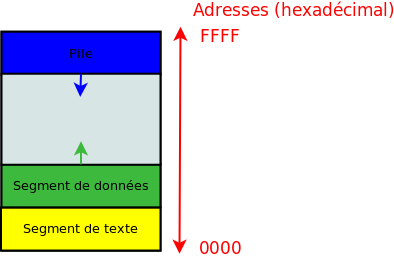
\includegraphics[scale=0.8]{img/adr.png}\end{center}
		\end{frame}	
		
	\subsection{Processus sous UNIX}
		\begin{frame}[containsverbatim]
			Lorsqu'un processus est lancé, le système doit gérer la mémoire et l'allocation du processeur lui étant accordée. Il fait appel à l'\textit{\textbf{ordonnanceur}}.
			\\~\\
			Sous les autres systèmes d'exploitation, un processus est l'équivalent d'un nouveau programme, alors que sous UNIX ce n'est pas forcément le cas.
			\\~\\
			La commande \lstinline!ps! permet d'afficher ses propres processus en cours d'exécution. Pour afficher tous les processus en cours d'exécution, on utilise l'option \lstinline!aux! (a : processus de tous les utilisateurs, u : affichage détaillé, x : démons).
			\\~\\
			\textbf{PID :}
			\\~\\
			Chaque processus peut être identifié par son numéro de processus, ou PID (\textbf{\textit{Process IDentifier}}). Un numéro de PID est unique dans le système : il est impossible que deux processus aient un même PID au même moment.
			
		\end{frame}	
		
		\begin{frame}
			\textbf{Organisation des processus :}
			\\~\\
			Lorsque l'on crée un processus, on utilise une fonction qui permet de dupliquer le processus appelant. On distingue alors les deux processus par leur PID. Le processus appelant est alors nommé \textbf{processus père} et le nouveau processus \textbf{processus fils}. Quant on s'occupe du processus fils, le PID du processus père est noté \textbf{PPID} (\textbf{\textit{Parent PID}}).
			\\~\\
			-> Les processus sont organisés en \textbf{\textit{hiérarchie}}.
			\\~\\
			\textbf{États d'un processus :}~\\
			\begin{itemize}
				\item exécution (R pour running) : le processus est en cours d'exécution
				\item sommeil (S pour sleeping) : dans un multitâche coopératif, quand il rend la main, ou dans un multitâche préemptif, quand il est interrompu au bout d'un quantum de temps
				\item arrêt (T pour stopped) : le processus a été temporairement arrêté par un signal, il ne s'exécute plus et ne réagira qu'à un signal de redémarrage
				\item zombie (Z pour … zombie) : le processus fils (zombie) s'est terminé avant le père
			\end{itemize}
		\end{frame}
		
		\begin{frame}
			\begin{center}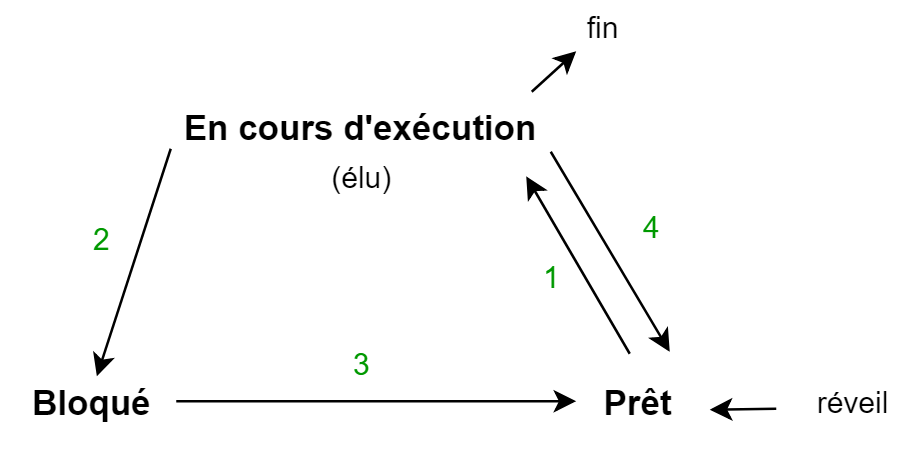
\includegraphics[scale=0.3]{img/process.png}\end{center}
			
			\begin{itemize}
				\item 1 : élection, l'ordonnanceur choisit ce processus
				\item 2 : blocage, processus bloqué en attente d'une donnée
				\item 3 : déblocage, donnée devient disponible
				\item 4 : l'ordonnanceur choisit un autre processus
			\end{itemize}
		\end{frame}	
		
	\subsection{Manipulation des processus en C}
		\begin{frame}[containsverbatim]
			\textbf{Création d'un processus :}
			\\~\\
			\begin{lstlisting}
				#include <unistd.h>
				#include <sys/types.h>

				pid_t fork(void);
			\end{lstlisting}
			Le processus d'origine est le processus père et le nouveau processus créé est le processus fils, qui possède un nouveau PID. Les processus deux ont le même code source, mais la valeur retournée par \lstinline!fork! nous permet de savoir si l'on est dans le processus père ou dans le processus fils. Ceci permet de faire deux choses différentes dans le processus père et le processus fils.
			\\~\\
			\noindent La fonction \lstinline!fork! retourne :
			\begin{itemize}
				\item -1 en cas d'erreur
				\item 0 si on est dans le processus fils
				\item le PID du fils si on est dans le processus père. Cela permet ainsi au père de connaître le PID de son fils
			\end{itemize}
		
		\end{frame}	
		
		\begin{frame}[containsverbatim]
			\noindent \textbf{Autres fonctions :}~\\
			\begin{lstlisting}
				#include <unistd.h>
				#include <sys/types.h>

				pid_t getpid(void);
				// retourne le PID du processus appelant
				
				pid_t getppid(void);
				// retourne le PPID du processus appelant
			\end{lstlisting}
		\end{frame}	
		
		\begin{frame}[containsverbatim]
			\textbf{Terminaison d'un processus :}\\~\\
			Un programme peut se terminer normalement de deux façons différentes. La plus simple consiste à laisser le processus finir le \lstinline!main! avec l'instruction \lstinline!return! suivie du code de retour du programme. Une autre façon est de terminer le programme grâce à la fonction \lstinline!exit()! depuis n'importe quelle fonction.
			\\~\\
			\begin{lstlisting}
				#include <stdlib.h>

				void exit(status);
			\end{lstlisting}
			~\\
			Un programme peut aussi se terminer de façon anormale, en cas d'erreur par exemple. Pour cela, on peut utiliser les fonctions \lstinline!abort(void)! ou \lstinline!assert(int condition)! par exemple. 
		\end{frame}	
		
		\begin{frame}[containsverbatim]
			\textbf{Synchronisation entre processus :}\\~\\
			Un processus \textbf{zombie} est un processus qui s'est achevé, mais qui dispose toujours d'un identifiant de processus (PID) et reste donc encore visible dans la table des processus. Lorsque le processus fils se termine avant le processus père (c'est à dire que le père n'a pas encore lu le code de retour du fils), le processus fils devient un zombie.
			\\~\\
			Pour permettre à un processus fils zombie de disparaître complètement, on utilise la fonction \lstinline!wait()!.\\
			\begin{lstlisting}
				#include <sys/types.h>
				#include <sys/wait.h>

				pid_t wait(int* status);
			\end{lstlisting}
			~\\
			Lorsque l'on appelle cette fonction, celle-ci bloque le processus à partir duquel elle a été appelée (père) jusqu'à ce qu'un de ses fils se termine. Elle renvoie alors le PID de ce dernier. En cas d'erreur, la fonction renvoie la valeur -1.
			\\~\\
			Le paramètre \lstinline!status! correspond au code de retour du processus (ce code de retour est généralement indiqué avec la fonction exit).\\
			Il faut veiller à mettre autant de \lstinline!wait! dans le père qu'il a de processus fils.\\
		\end{frame}	
		
		\begin{frame}[containsverbatim]
			\textbf{La fonction \lstinline!waitpid! :} 
			\\~\\
			Permet de suspendre l'exécution d'un processus père jusqu'à ce qu'un de ses fils, dont on doit passer le PID en paramètre, se termine.~\\
			\begin{lstlisting}
				#include <sys/wait.h>

				pid_t waitpid(pid_t pid, int* status, int options);
				\\waitpid(-1, status, 0) correspond à wait
			\end{lstlisting}
			~\\
			\begin{itemize}
				\item si pid > 0, le processus père est suspendu jusqu'à la fin d'un processus fils dont le PID est égal à la valeur pid
				\item si pid = 0, le processus père est suspendu jusqu'à la fin de n'importe lequel de ses fils appartenant à son groupe
				\item si pid = -1, le processus père est suspendu jusqu'à la fin de n'importe lequel de ses fils
				\item si pid < -1, le processus père est suspendu jusqu'à la mort de n'importe lequel de ses fils dont le GID est égal
				\item \lstinline!status! a le même rôle qu'avec \lstinline!wait!
				\item \lstinline!options! permet de préciser le comportement de \lstinline!waitpid!
			\end{itemize}
		\end{frame}	
		
		\begin{frame}
			\begin{center}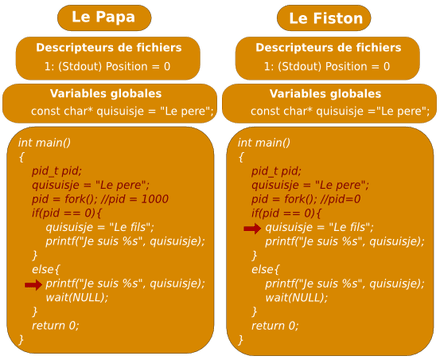
\includegraphics[scale=0.6]{img/fork1.png}\end{center}
		\end{frame}	
		
		\begin{frame}
			\begin{center}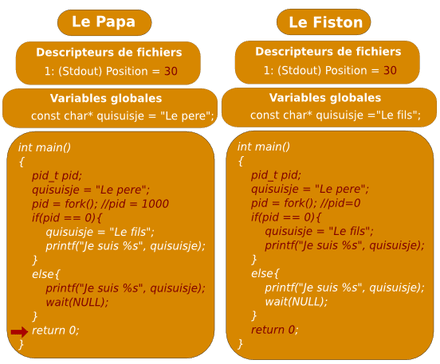
\includegraphics[scale=0.6]{img/fork2.png}\end{center}
		\end{frame}	
		
		\begin{frame}[containsverbatim]
			La variable \lstinline!quiSuisJe! va être modifiée pour le processus fils seulement. La position de \lstinline!stdout! va avancer de 15 caractères pour le \lstinline!printf! du père et 15 autres caractères pour le \lstinline!printf! du fils pour valoir 30 au final pour les deux processus.
			\\~\\
			Les variables du processus père et celles du fils sont totalement distinctes. Par contre, leur descripteurs de fichiers sont les mêmes. Donc, si l'un des deux processus modifie son pointeur de position dans un fichier, ça se répercutera également chez l'autre. Cela ne vaut que pour les descripteurs de fichiers hérités durant le \lstinline!fork!, c'est-à-dire, si le père ou le fils ouvre d'autres fichiers après le \lstinline!fork!, ces descripteurs ne seront pas partagés entre eux deux. De même, si le fils ferme un descripteur de fichier hérité du père, le descripteur de fichier du père ne sera par contre pas fermé (même chose dans le sens inverse).
			\\~\\
			\noindent On ne peut pas savoir quel processus va s'exécuter en premier. Pour la fonction \lstinline!wait!, il est préférable l'utiliser ainsi :
			\begin{lstlisting}
				if ( wait(NULL) == -1 )
					perror("wait");
			\end{lstlisting}
				
		
		\end{frame}	
		
	\section{Threads}
		\begin{frame}
			Un \textbf{thread} ou \textbf{fil (d'exécution)} ou \textbf{tâche} (aussi processus léger) représente, comme un processus, l'exécution d'un ensemble d'instructions du langage machine d'un processeur. Du point de vue de l'utilisateur, ces exécutions semblent se dérouler en parallèle. Toutefois, là où chaque processus possède sa propre mémoire virtuelle, les threads d'un même processus se partagent sa mémoire virtuelle. Par contre, tous les threads possèdent leur propre pile d'exécution.
			\\~\\
			Dans la plupart des systèmes d'exploitation, chaque processus possède un espace d'adressage et un thread de contrôle unique, le thread principal. Du point de vue programmation, ce dernier exécute le \lstinline!main!.
			\\~\\
			En général, le système réserve un processus à chaque application, sauf quelques exceptions. Beaucoup de programmes exécutent plusieurs activités en parallèle, du moins en pseudo-parallélisme. Comme à l'échelle des processus, certaines de ces activités peuvent se bloquer, et ainsi réserver ce blocage à un seul thread séquentiel, permettant par conséquent de ne pas stopper toute l'application.
		\end{frame}	
		
	\subsection{Manipulation des threads en C}
		\begin{frame}[containsverbatim]
			\textbf{Créer un thread :}
			\\~\\
			Pour créer un thread, il faut déjà déclarer une variable le représentant. Celle-ci sera de type \lstinline!pthread_t!. Ensuite, pour créer la tâche elle-même, il suffit d'utiliser la fonction :
			\begin{lstlisting}
				#include <pthread.h>

				int pthread_create(pthread_t* thread, pthread_attr_t * attr, void* (*start_routine) (void*), void* arg);
			\end{lstlisting}
			\begin{itemize}
				\item retour : 0 si la création a été réussie ou une autre valeur si il y a eu une erreur
				\item \lstinline!thread! : pointeur vers l'identifiant du thread à créer
				\item \lstinline!attr! : attributs du thread, possible de mettre le thread en état joignable (NULL par défaut) ou détaché, et choisir sa politique d'ordonnancement (usuelle, temps-réel...)
				\item \lstinline!(*start_routine) (void*)! : pointeur vers la fonction à exécuter dans le thread, de la forme \lstinline!void* fonction(void* arg)! et contiendra le code à exécuter par le thread
				\item \lstinline!arg! : l'argument à passer au thread
			\end{itemize}
		\end{frame}
		
		\begin{frame}[containsverbatim]
			\textbf{Supprimer un thread :}
			\\~\\
			\begin{lstlisting}
				#include <pthread.h>

				void pthread_exit(void* ret);
			\end{lstlisting}
			Prend en argument la valeur qui doit être retournée par le thread, et doit être placée en dernière position dans la fonction concernée.
			\\~\\
			\textbf{Attendre la fin d'un thread :}
			\\~\\
				Le thread principal n'attendra pas que le thread créé termine de s'exécuter. La fonction \lstinline!pthread_join! pour cela.
				\begin{lstlisting}
					#include <pthread.h>

					int pthread_join(pthread_t th, void **thread_return);
				\end{lstlisting}
				Elle prend en premier paramètre l'identifiant du thread et son second paramètre, un pointeur, permet de récupérer la valeur retournée par la fonction dans laquelle s'exécute le thread (c'est-à-dire l'argument de \lstinline!pthread_exit!).
		\end{frame}
		
		\begin{frame}[containsverbatim]
			\begin{lstlisting}
				void* thread_1(void *arg) {
					printf("Nous sommes dans le thread.\n");
					pthread_exit(NULL);
				}

				int main(void) {
					pthread_t thread1;

					printf("Avant la création du thread.\n");

					if (pthread_create(&thread1, NULL, thread_1, NULL)) 
					{
						perror("pthread_create");
						return EXIT_FAILURE;
					}
					
					// on attend que le thread s'exécute
					if (pthread_join(thread1, NULL)) 
					{
						perror("pthread_join");
						return EXIT_FAILURE;
					}

					printf("Après la création du thread.\n");

					return EXIT_SUCCESS;
				}
			\end{lstlisting}
		\end{frame}	
		
	\subsection{Exclusions mutuelles}
		\begin{frame}[containsverbatim]
			Avec les threads, toutes les variables sont partagées (mémoire partagée). Cela pose des problèmes quand deux threads cherchent à modifier deux variables en même temps. Les mutex est mécanisme de synchronisation, un des outils permettant l'exclusion mutuelle.
			\\~\\
			Un \textbf{mutex} en C est une variable de type \lstinline!pthread_mutex_t!. Elle va nous servir de verrou, pour nous permettre de protéger des données. Ce verrou peut donc prendre deux états : disponible et verrouillé.
			\\~\\
			Quand un thread a accès à une variable protégée par un mutex, on dit qu'il tient le mutex. Il ne peut y avoir qu'un seul thread qui tient le mutex en même temps.
			\\~\\
			Le mutex doit être accessible en même temps que la variable et dans tout le fichier (vu que différents threads s'exécutent dans différentes fonctions). La solution la plus simple consiste à déclarer les mutex en variable globale.
		\end{frame}
		
		\begin{frame}[containsverbatim]
			\textbf{Initialiser un mutex :}
			\\~\\
			On initialise un mutex avec la valeur de la constante \lstinline!PTHREAD_MUTEX_INITIALIZER!, déclarée dans \lstinline!pthread.h!.
			\begin{lstlisting}
				#include <pthread.h>

				pthread_mutex_t mutex = PTHREAD_MUTEX_INITIALIZER;
			\end{lstlisting}
			~\\
			\textbf{Verrouiller un mutex :}
			\\~\\
			L'étape suivante consiste à établir une \textbf{zone critique}, c'est-à-dire la zone où plusieurs threads risquent de modifier ou de lire une même variable en même temps. On verrouille donc le mutex pour éviter ce risque.
			\begin{lstlisting}
				#include <pthread.h>

				int pthread_mutex_lock(pthread_mutex_t *mut);
			\end{lstlisting}
		\end{frame}
		
		\begin{frame}[containsverbatim]
			\textbf{Déverrouiller un mutex :}
			\\~\\
			À la fin de la zone critique, il suffit de déverrouiller le mutex.
			\begin{lstlisting}
				#include <pthread.h>

				int pthread_mutex_unlock(pthread_mutex_t *mut);
			\end{lstlisting}
			~\\
			\textbf{Détruire un mutex :}
			\\~\\
			Une fois le travail du mutex terminé, on peut le détruire.
			\\~\\
			\begin{lstlisting}
				#include <pthread.h>

				int pthread_mutex_destroy(pthread_mutex_t *mut);
			\end{lstlisting}
		\end{frame}
		
		\begin{frame}[containsverbatim]
			\textbf{Les conditions :}
			\\~\\
			Lorsqu'un thread doit patienter jusqu'à ce qu'un événement survienne dans un autre thread, on utilise les conditions.\\
			Quand un thread est en attente d'une condition, il reste bloqué tant que celle-ci n'est pas réalisée par un autre thread.
			\\~\\
			Comme avec les mutex, on déclare la condition en variable globale :
			\begin{lstlisting}
				pthread_cond_t nomCondition = PTHREAD_COND_INITIALIZER;
			\end{lstlisting}
			~\\
			Pour attendre une condition, il faut utiliser un mutex :
			\begin{lstlisting}
				int pthread_cond_wait(pthread_cond_t *nomCondition, pthread_mutex_t *nomMutex);
			\end{lstlisting}
			~\\
			Pour réveiller un thread en attente d'une condition, on utilise la fonction :
			\begin{lstlisting}
				int pthread_cond_signal(pthread_cond_t *nomCondition);
			\end{lstlisting}
		\end{frame}	
		
		\begin{frame}
			Créez un code qui crée deux threads : un qui incrémente une variable compteur par un nombre tiré au hasard entre 0 et 10, et l'autre qui affiche un message lorsque la variable compteur dépasse 20.
		\end{frame} 
		
		\begin{frame}[containsverbatim]
			\begin{lstlisting}
				#include <stdio.h>
				#include <stdlib.h>
				#include <pthread.h>

				pthread_cond_t condition = PTHREAD_COND_INITIALIZER;
				pthread_mutex_t mutex = PTHREAD_MUTEX_INITIALIZER;

				void* threadAlarme (void* arg);
				void* threadCompteur (void* arg);

				int main (void)
				{
					pthread_t monThreadCompteur;
					pthread_t monThreadAlarme;

					pthread_create (&monThreadCompteur, NULL, threadCompteur, (void*)NULL);
					pthread_create (&monThreadAlarme, NULL, threadAlarme, (void*)NULL);

					pthread_join (monThreadCompteur, NULL);
					pthread_join (monThreadAlarme, NULL);

					return 0;
				}
			\end{lstlisting}
		\end{frame}
		
		\begin{frame}[containsverbatim]
			\begin{lstlisting}
				void* threadCompteur (void* arg)
				{
					int compteur = 0, nombre = 0;
					srand(time(NULL));

					while(1) {
						nombre = rand()%10; /* On tire un nombre entre 0 et 10 */
						compteur += nombre; /* On ajoute ce nombre à la variable compteur */

						printf("\n%d", compteur);
						
						if(compteur >= 20) /* Si compteur est plus grand ou égal à 20 */
						{
							pthread_mutex_lock (&mutex); /* On verrouille le mutex */
							pthread_cond_signal (&condition); /* On délivre le signal : condition remplie */
							pthread_mutex_unlock (&mutex); /* On déverrouille le mutex */

							compteur = 0; /* On remet la variable compteur à 0 */
						}
						sleep (1); /* On laisse 1 seconde de repos */
					}
					pthread_exit(NULL); /* Fin du thread */
				}
			\end{lstlisting}
		\end{frame}
		
		\begin{frame}[containsverbatim]
			\begin{lstlisting}
				void* threadAlarme (void* arg)
				{
					while(1) /* Boucle infinie */
					{
						pthread_mutex_lock(&mutex); /* On verrouille le mutex */
						pthread_cond_wait (&condition, &mutex); /* On attend que la condition soit remplie */
						printf("\nLE COMPTEUR A DÉPASSÉ 20."); 
						pthread_mutex_unlock(&mutex); /* On déverrouille le mutex */
					}
					
					pthread_exit(NULL); /* Fin du thread */
				}
			\end{lstlisting}
		\end{frame}
\end{document}
